% #region PREAMBEL OG PAKKER
\documentclass[a4paper, 12pt]{article}  % DOKUMENTKLASSE
\title{Øving 9}               % TITTEL
\author{Håvard Solberg Nybøe}           % FORFATTER
\date{MA0001 -- \today}                    % DATO & FAG

\usepackage[english, norsk]{babel}      % NORSK SPRÅK
\usepackage[
    backend=biber,style=apa]{biblatex}  % BIBLIOGRAFI
\usepackage{csquotes}                   % PAKKE TIL BABEL
\addbibresource{bibliografi.bib}        % PATH TIL BIBLIOGRAFI
\usepackage[hidelinks]{hyperref}        % LENKER I TOC OG GENERELT
\usepackage[margin=1in]{geometry}       % VANLIG STØRRELSE MARGIN
\setlength{\parindent}{0em}             % SKILLER AVSNITT
\setlength{\parskip}{.8em}              % SKILLER AVSNITT
\usepackage{graphicx, float}            % BILDER \includegraphics[OPTIONS]{PATH}
\usepackage{kantlipsum}                 % FYLLTEKST I KANT-STIL (kant[n-m])
\usepackage{amsfonts,amsmath,amssymb}   % BLACKBOARD BOLD FONT (\mathbb{N}) & SYMBOLER
\usepackage{circuitikz,pgfplots}        % LOGISKE PORTER OG KRETSER & TikZ
\usetikzlibrary{shapes.geometric}       % STILER TIL FLYTSKJEMA
\tikzstyle{startstop} = [rectangle, rounded corners, minimum width=3cm, minimum height=1cm, text centered, draw=black, fill=red!30]
\tikzstyle{io} = [trapezium, trapezium left angle=70, trapezium right angle=110, minimum width=3cm, minimum height=1cm, text centered, draw=black, fill=blue!30]
\tikzstyle{prosess} = [rectangle, minimum width=3cm, text width=3cm, minimum height=1cm, text centered, draw=black, fill=orange!30]
\tikzstyle{decision} = [diamond, minimum width=3cm, minimum height=1cm, text centered, draw=black, fill=green!30]
\tikzstyle{arrow} = [thick, ->, > = stealth]
% #endregion
\begin{document}

\maketitle
% \tableofcontents % INNHOLDSFORTEGNELSE

\begin{enumerate}
    \item [\boxed{1}]
          \begin{align*}
              f: \mathbb{R} \rightarrow \mathbb{R}, \quad & \quad f(x) = \frac{x}{e^x}                                  \\
              f'(x)                                       & = \frac{-x+1}{e^x}                                          \\
              \frac{-x+1}{e^x}                            & = \frac{-x}{e^x} + \frac{1}{e^x}                            \\
              \text{Finner null}                          & \text{punktet til } f'(x)                                   \\
              \frac{-x}{e^x} + \frac{1}{e^x}              & = 0                                                         \\
              \frac{x}{e^x}                               & = \frac{1}{e^x}                                             \\
              x                                           & = 1                                                         \\
              f(1)                                        & = \frac{1}{e}                                               \\
              \text{Funksjonen } f                        & \text{ har ett ekstremalpunkt} = \left(1, {1\over e}\right) \\
          \end{align*}
    \item [\boxed{2}]
          \begin{align*}
              g: \mathbb{R} \rightarrow \mathbb{R}, \quad    & \quad g(x) = x^4 - 10x^3 + x^2 + 4x -2              \\
              g'(x)                                          & = 4x^3 - 30x^2 + 2x + 4                             \\
              \text{Finner null}                             & \text{punktene til } g'(x)                          \\
              4x^3 - 30x^2 + 2x + 4                          & = 0                                                 \\
              x = -0.33 \land x                              & = 0.41 \land  x = 7.41                              \\
              \text{Funksjonen } g                           & \text{ er konveks/konkav i intervallene}            \\
                                                             & \Downarrow                                          \\
              x \in [-\infty, 0.33) \land x \in (0.33, 0.41) & \land x \in (0.41, 7.41) \land x \in (7.41, \infty] \\
          \end{align*}
    \item [\boxed{3}]
    \item [\boxed{4}] \textbf{ }
          \begin{figure}[H]
              \begin{center}
                  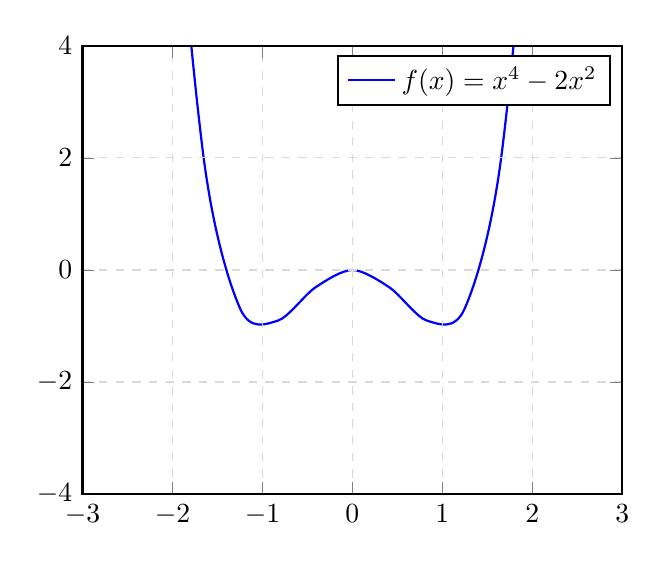
\begin{tikzpicture}
                      \begin{axis}[ymin=-4, ymax=4, xmin=-3, xmax=3, axis on top, style=thick, grid, grid style={dashed,gray!30}]
                          \addplot[color=blue, smooth]{x^4-2*x^2};
                          \addlegendentry{$f(x) = x^4-2x^2 $};
                      \end{axis}
                  \end{tikzpicture}
              \end{center}
          \end{figure}
\end{enumerate}

% \printbibliography[heading=bibintoc] % LAGER BIBLIOGRAFI
\end{document}